\documentclass[12pt,a4paper,twoside]{article}

\usepackage[utf8]{inputenx}
\usepackage[T1]{fontenc}

\usepackage[
	spanish,
	es-minimal
]{babel}
\unaccentedoperators

\usepackage{solutions}
\usepackage{choices}

\usepackage{lipsum}
\usepackage{graphicx}

\usepackage{amsmath}
\usepackage{amsthm}
\usepackage{amssymb}

\usepackage{mymedia}
\usepackage{hyperref}

\title{De LaTeX a HTML}
\author{Nombre español}

\newtheorem{theorem}{Theorem}
\newtheorem{corollary}[theorem]{Corollary}
\newtheorem{lemma}[theorem]{Lemma}
\newtheorem{definition}[theorem]{Definition}
\begin{document}

\maketitle

\tableofcontents



\section{Introducción}
Documento basado en muestra proporcionada por Prof. Toby Roberts (disponible \href{http://www.maths.adelaide.edu.au/anthony.roberts/LaTeX/Src/maths.tex}{aquí}).

AQUÍ VA EL TEXTO CON LA INTRODUCCIÓN
 
\subsection{Organiza tus ideas}
 AQUÍ VA EL ESQUEMA DEL LIBRO

\section{Concepto de función}

\begin{definition}
Una \emph{correspondencia} es una relación entre dos conjuntos tal que a cada elemento del primer conjunto le corresponde ninguno, uno o varios elementos del segundo conjunto.
\end{definition}

A continuación, se muestra un ejemplo de correspondencia entre personas y sus respectivos números de DNI.

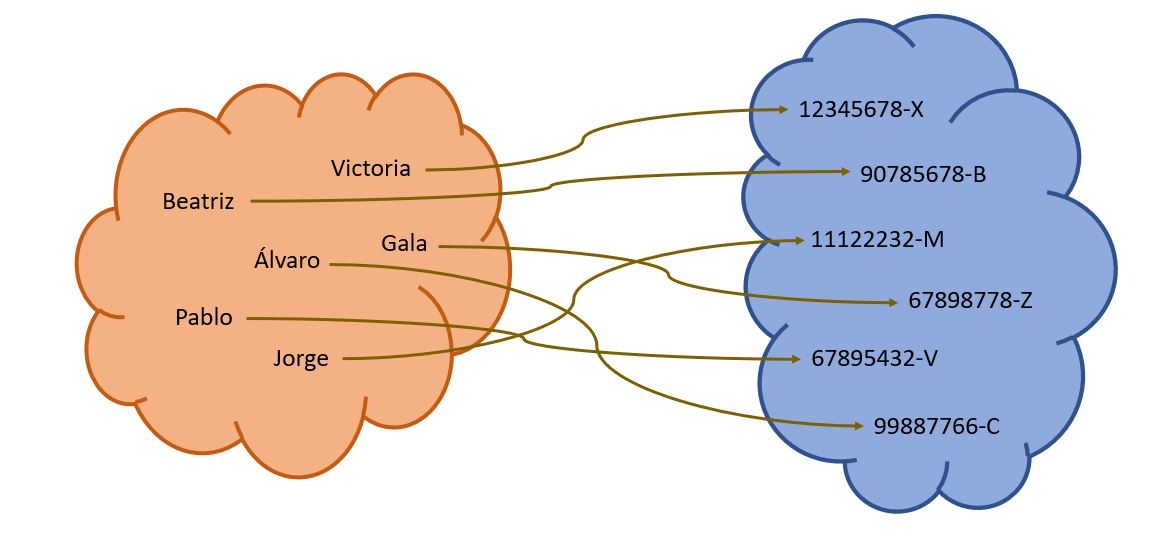
\includegraphics{samples/imagenes/imagenConcepto.jpg}

\begin{definition}
Una \emph{función} es una correspondencia tal que a cada valor del primer conjunto le corresponde un único valor del segundo conjunto. 
\end{definition}
\geogebra{bm9zpgfh}
Un ejemplo claro de función podría ser la relación existente entre un hijo y su madre, ya que cada hijo tiene una única madre.

Existen diferentes formas de expresar una función:
\begin{itemize}
	\item \emph{Mediante un enunciado verbal.}
	\item \emph{Mediante una gráfica.}
	\item \emph{Mediante una fórmula matemática.}
	\item \emph{Mediante una fórmula matemática.}
\end{itemize}

\subsubsection{Ejercicios.}
\begin{enumerate}
	\item Introduzca en la barra de entrada las siguientes funciones, de manera similar a la indicada en el ejemplo anterior, y observa la gráfica de representación de cada una de las funciones.\\
	\begin{itemize}
		\item $f(x) = 3x+2$
		\item $g(x) = \dfrac{x^2-3}{x+5}$
		\item $h(x) = \sqrt{x+5}$
		\item $j(x) = \dfrac{2x^2+1}{3x-5}$
		\item $k(x) = \log (x^2)$
		\item $p(x) = 3\cos(3x)$
	\end{itemize}
	\geogebra[ai=true, stb=true]{tc5pbmae}
	\item Cite todas las familias de funciones a las que pertenecen cada una de las siguientes:
	\begin{itemize}
		\item $f(x) = 2x^3-3x$
		\item $f(x) = 6x+2$
		\item $f(x) = -\sqrt{x+1}$
		\item $f(x) = \tan (x-4)$
		\item $f(x) = \dfrac{2x-1}{x+7}$
		\item $f(x) = \log(x^2)$
	\end{itemize}

\end{enumerate}

\begin{ex}[sol after]
	Enunciado ejercicio.
	\lipsum[1]
	\begin{sol}
		Solución a continuación.
		\lipsum[1]
	\end{sol}
\end{ex}


\section{Operaciones con funciones}

Sean dos funciones $f$ y $g$ definidas en el mismo subconjunto $D$ de los números reales, se definen las siguientes operaciones entre ellas:
\begin{itemize}
	\item \textbf{Adición}: la suma de $f$ y $g$ es la función $f+g$ que, para cualquier $x \in D$, verifica:
	$$(f+g)(x) = f(x)+g(x)$$
	\item \textbf{Sustracción}: la diferencia de $f$ y $g$ es la función $f-g$ que, para cualquier $x \in D$, verifica:
	$$(f-g)(x) = f(x)-g(x)$$
	\item \textbf{Multiplicación}: el producto de $f$ y $g$ es la función $f \cdot g$ que, para cualquier $x \in D$, verifica:
	$$(f \cdot g)(x) = f(x) \cdot g(x)$$
	\item \textbf{División}: el cociente de $f$ y $g$ es la función $\frac{f}{g}$ que, para cualquier $x \in D$, con $g(x) \neq 0$, verifica:
	$$(\dfrac{f}{g})(x) = \dfrac{f(x)}{g(x)}$$
\end{itemize}
Las operaciones con funciones verifican las mismas propiedades que las operaciones con números reales, ya que se definen utilizando las operaciones con sus imágenes, que son números reales.\\
El dominio de las funciones $f+g$, $f-g$, $f \cdot g$ y $\dfrac{f}{g}$ es la intersección de los dominios de $f$ y $g$, con la salvedad de que en el caso $\dfrac{f}{g}$, los valores de x que anulan el denominador no pertenecen al dominio.\\

EJEMPLO
\youtube{jP1mSfUqpxw}

\subsubsection{Ejercicios}

\begin{ex}[sol later]
	Dadas las funciones $f(x)=5x+6$ y $g(x)=3x^2-4x+8$, calcula la suma $(f+g)(x)$ y la resta $(f-g)(x)$ de las funciones.
	\begin{sol}
		\begin{itemize}
			\item $(f+g)(x) = f(x)+g(x) = (5x+6)+(3x^2-4x+8) = 3x^2+x+14$
			\item $(f-g)(x) = f(x)-g(x) = (5x+6)-(3x^2-4x+8) = -3x^2+9x-2$
		\end{itemize}
	\end{sol}
\end{ex}

\vspace{1cm}

\begin{ex}[sol later]
	Dadas las funciones $f(x)=12x^3+15x^2-6x$ y $g(x)=3x$, calcula el producto $(f \cdot g)(x)$ y la división $(\dfrac{f}{g})(x)$ de las funciones.
	\begin{sol}
		\begin{itemize}
			\item $(f \cdot g)(x) = f(x) \cdot g(x) = (12x^3+15x^2-6x) \cdot(3x) = 36x^4+45x^3-18x^2$
			\item $(\dfrac{f}{g})(x) = \dfrac{f(x)}{g(x)} = \dfrac{(12x^3+15x^2-6x)}{(3x)} = 4x^2+5x-2$
		\end{itemize}
	\end{sol}
\end{ex}

\vspace{1cm}

\begin{ex}[sol later]
	Dadas las funciones $f(x)=\sqrt{x}$, $g(x)=x-4$ y $h(x)=\dfrac{2}{3-x}$, calcula $(f+g)(x), (g+h)(x), (\dfrac{f}{g})(x), (\dfrac{g}{f})(x), (f\cdot g)(x)$ y $(\dfrac{g}{h})(x)$.
	\begin{sol}
		\begin{itemize}
			\item $(f+g)(x) = f(x) + g(x) = \sqrt{x} + (x-4) = \sqrt{x} + x -4$
			\item $(g+h)(x) = g(x) + h(x) = (x-4) + \dfrac{2}{3-x} = x - 4 + \dfrac{2}{3-x}$
			\item $(\dfrac{f}{g})(x) = \dfrac{f(x)}{g(x)} = \dfrac{\sqrt{x}}{x-4}$
			\item $(\dfrac{g}{f})(x) = \dfrac{g(x)}{f(x)} = \dfrac{x-4}{\sqrt{x}}$
			\item $(f\cdot g)(x) = f(x) \cdot g(x) = \sqrt{x} \cdot \dfrac{2}{3-x} = \dfrac{2\sqrt{x}}{3-x}$
			\item $(\dfrac{g}{h})(x) = \dfrac{g(x)}{h(x)} = \dfrac{x-4}{\dfrac{2}{3-x}} = \dfrac{(x-4)(3-x)}{2}$
		\end{itemize}
	\end{sol}
\end{ex}


\section{Función compuesta}

\begin{definition}
Dadas dos funciones $f$ y $g$, la \emph{función compuesta} de $f$ y $g$, que se simboliza con $g \circ f$, es la función que transforma $x$ en $g(f(x))$.
$$ x \rightarrow f(x) \rightarrow g(f(x))$$
El dominio de la función compuesta $g \circ f$ está formada por los valores de $x$ pertenecientes al dominio de $f$ tales que $f(x)$ pertenece al dominio de $g$.
\end{definition}
Por ejemplo, si $f(x) = 3x - 1$ y $g(x) = \dfrac{1}{x^{2}+1}$, entonces la función compuesta $f$ y $g$ es $$(g \circ f)(x) = g(f(x)) = g(3x-1) = \dfrac{1}{(3x-1)^{2}+1}$$.\\
También podemos considerar la función compuesta de $g$ y $f$:
$$(f \circ g)(x) = f(g(x)) = f(\dfrac{1}{x^2 + 1}) = 3 \cdot \dfrac{1}{x^2 + 1} - 1$$
En general, la composición de funciones no es una operación conmutativa. Es decir, $g \circ f \neq f \circ g$, excepto en algunos casos particulares. Además, se puede dar el caso de que alguna de las dos funciones compuestas no exista.
\youtube{v8j1qoTvDSg}

\begin{ex}[sol later]
	Sean $f(x)=3x+2$ y $g(x)=\dfrac{x+3}{2x+1}$, calcula $(g \circ f)$ y $(f \circ g)$.
	\begin{sol}
		\begin{itemize}
			\item $g \circ f = g[f(x)] = g(3x+2) = \dfrac{3x+2+3}{2(3x+2)+1} = \dfrac{3x+5}{6x+5}$
			\item $f \circ g = f[g(x)] = f(\dfrac{x+3}{2x+1}) = 3\dfrac{x+3}{2x+1} + 2=\dfrac{7x+11}{2x+1}$
		\end{itemize}
	\end{sol}
\end{ex}

\vspace{1cm}


\begin{ex}[sol later]
	Sean $f(x)=\dfrac{x+2}{2x+1}$ y $g(x)=\sqrt{x}$, calcula $g \circ f$ y $f \circ g$.
	\begin{sol}
		\begin{itemize}
			\item $g \circ f = g[f(x)] = g(\dfrac{x+2}{2x+1}) = \sqrt{\dfrac{x+2}{2x+1}}$
			\item $f \circ g = f[g(x)] = f(\sqrt{x}) =\dfrac{\sqrt{x}+2}{2\sqrt{x}+1}$
		\end{itemize}
	\end{sol}
\end{ex}

\vspace{1cm}

\begin{ex}[sol later]
	Sean $f(x)=\dfrac{1}{2x-1}$, $g(x)=\dfrac{2x-1}{2x+1} \text{ y } h(x)=\dfrac{1}{x}$, calcula $g \circ f$, $f \circ g$, $h \circ g \circ f$ y $h \circ f \circ g$.
	\begin{sol}
		\begin{itemize}
			\item $g \circ f = g[f(x)] = g(\dfrac{1}{2x-1}) = \dfrac{2(\dfrac{1}{2x-1})-1}{2(\dfrac{1}{2x-1})+1} = \dfrac{3-2x}{2x+1}$
			\item $f \circ g = f[g(x)] = f(\dfrac{2x-1}{2x+1}) =\dfrac{1}{2(\dfrac{2x-1}{2x+1})-1} = \dfrac{2x+1}{2x-3}$
			\item $h \circ g \circ f= h[(g \circ f)(x)] = h(\dfrac{3-2x}{2x+1}) = \dfrac{2x+1}{3-2x}$
			\item $h \circ f \circ g= h[(f \circ g)(x)] = h(\dfrac{2x+1}{2x-3}) = \dfrac{2x-3}{2x+1}$
		\end{itemize}
	\end{sol}
\end{ex}



\section{Función inversa de una función}

\begin{definition}
Dada una función $f$, se denomina \emph{función inversa} de $f$, si existe, y se simboliza con $f^{-1}$, la función que cumple:
$$f^{-1}(y) = x \longleftrightarrow f(x) = y$$
\end{definition}
La función inversa de $f^{-1}$ es, a su vez, $f: (f^{-1})^{-1}=f$.Por eso decimos, simplemente, que las funciones f y f^{-1} son inversas.
La composición de una función $f$ con su inversa $f^{-1}$ es la \emph{función identidad}, $I(x)=x$:
$$(f^{-1} \circ f)(x) = f^{-1}(f(x)) = I(x)$$
$$(f \circ f^{-1})(x) =f(f^{-1}(x))=I(x)$$

\subsubsection{Obtención de la función inversa}
Para calcular la función inversa de una función dada $f$ debemos de seguir el siguiente procedimiento:
\begin{enumerate}
	\item Se escribe la función con $x$ e $y$.
	\item Se despeja la variable $x$ en función de la variable $y$.
	\item Se intercambian las variables.
\end{enumerate}
\youtube{l6pZGhy0hHc}

\subsubsection{Ejercicios}
\begin{ex}[sol after]
	Halla la función inversa de $f(x)=2x+3$.
	\begin{sol}
		\begin{enumerate}
			\item Intercambiamos las variables $x$ e $y$ en la expresión $y=2x+3$, con lo que resulta $x=2y+3$.
			\item Despejamos $y$, con lo que obtenemos $y=\dfrac{x-3}{2}$. Luego $f^{-1}(x)=\dfrac{x-3}{2}$.
			\item Comprobamos que la composición de las dos funciones hace corresponder a cada $x$ el mismo $x$:
			$$(f^{-1} \circ f)(x) = f^{-1}(f(x)) = f^{-1}(2x+3) = \dfrac{2x + 3 - 3}{2} = x$$
			$$(f \circ f^{-1})(x) = f(f^{-1}(x)) = f(\dfrac{x-3}{2}) =2 \cdot \dfrac{x-3}{2} + 3 = x$$
		\end{enumerate}
	\end{sol}
\end{ex}

\vspace{1cm}

\begin{ex}[sol later]
	En cada caso, calcula la función inversa de la dada:\\
	\begin{itemize}
		\item $f(x) = x^2 -\dfrac{1}{2}$
		\item $h(x) = \log (x)$
		\item $j(x) = \sqrt{x^2+5}$
	\end{itemize}
	\begin{sol}
		\begin{itemize}
			\item $f^{-1}(x) = \sqrt{\dfrac{2x+1}{2}}$
			\item $h^{-1} = e^{x}$
			\item $j^{-1} = \sqrt{x^2-5}$
		\end{itemize}
	\end{sol}
\end{ex}

\section{Propiedades globales de una función}

\subsection{Dominio}

\begin{definition}
	El \emph{dominio de una función real}, también llamado \textbf{dominio de definición} o \textbf{campo de existencia}, es el conjunto de los elementos para los cuales la función está definida. Dicho de otra manera, es el subconjunto de números reales que tienen imagen.
	$$Dom_{f} =\{x \in R / \exists y = f(x) \in \mathbb{R}\}$$
\end{definition}
\begin{itemize} 
	\item $Dom_{f}$: dominio de la función. También se puede denotar por $Dom(f)$ o, simplemente, $D$. Puede ser todo el conjunto de los números reales, o buen un subconjunto de este: $Dom_{f} \subseteq R$. 
	\item $x$: número real, perteneciente al dominio de la función, que recibe el nombre de variable independiente. 
	\item $y$: número real, perteneciente al conjunto e la imagen de la función, recibe el nombre de variables dependiente. Para obtener su valor se debe aplicar la función $f$ al valor de $x: f(x)=y$. Para un par de valores concretos $(x,y)$ se dice que $y$ es la \textbf{imagen} de $x$, y que $x$ es la \textbf{antiimagen} de $y$.
\end{itemize} 
\youtube{lmfDEGDpgV8}
\subsubsection{Cómo calcular el dominio}
Para calcular el dominio "eliminaremos" de la ecuación aquellos valores que hagan imposible realizar alguna operación matemática.
\begin{itemize}
	\item \textbf{Funciones polinómicas}\\
	El dominio de toda función polinómica es R, ya que al sustituir un número real cualquiera $x \in R$, siempre va a existir $f(x)$.
	\item \textbf{Funciones racionales}\\
	El \textbf{denominador} debe de ser \textbf{diferente de cero}. Suponiendo una función $f(x) = \dfrac{P(x)}{Q(x)}$, si tanto $P(x)$ como $Q(x)$ son polinomios, entonces el dominio $Dom_{f}= \{x \in R / Q(x) \neq 0\}$, es decir, el conjunto de valores que \textbf{no anulan} el denominador.\\
	Cuando simplifiques una función racional, el dominio debe coincidir con el de la función original, y no debes caer en la tentación de recalcularlo.
	\item \textbf{Funciones irracionales}\\
	\begin{itemize}
		\item \emph{Función irracional de índice impar}\\
		En estos casos, la raíz no impone ninguna restricción adicional al dominio, por lo que coincidirá con el del radicando.
		\item \emph{Función irracional de índice par}\\
		En estos casos la raíz impone que los valores del radicando siempre sean mayores o iguales que cero.
	\end{itemize}
	\item \textbf{Funciones exponenciales}\\
	En estos casos, la exponencial no impone ninguna restricción adicional al dominio, con lo que coincidirá con el dominio del exponente.
	\item \textbf{Funciones logarítmicas}\\
	En estos casos el logaritmo impone que el argumento debe de ser un número positivo. 	
\end{itemize}
\subsubsection{Ejercicios}
\begin{ex}[sol later]
	Calcula el dominio de las siguientes funciones a partir de la teoría explicada previamente:\\
	\begin{itemize}
		\item $f(x) = \dfrac{2x}{3x-2}$
		\item $f(x) = \dfrac{6x}{x^2-16}$
		\item $f(x) = \sqrt{x^2-1}$
		\item $f(x) = \sqrt{\dfrac{3}{-x+2}}$
		\item $f(x) = \sqrt{\dfrac{x+5}{x-7}}$
		\item $f(x) = \sqrt{x^2+x}$
		\item $f(x) = \log(-2x^2-10x-8)$
		\item $f(x) = \arccos(x+5)$
		\item $f(x) = e^x$
		\item $f(x) = e^{-5x}$
	\end{itemize}
	\begin{sol}
		\begin{itemize}
			\item $\mathbb{R}-\{\dfrac{2}{3}\}$
			\item $\mathbb{R}-\{-4, 4\}$
			\item $(-\infty, -1]\bigcup [1, +\infty])$
			\item $(-\infty, 2)$
			\item $(-\infty, -5]\bigcup [7, +\infty])$
			\item $(-\infty, -1]\bigcup [0, +\infty])$
			\item $(-4,-1)$
			\item $[-6, -4]$
			\item $\mathbb{R}$
			\item $\mathbb{R}$
		\end{itemize}
	\end{sol}
\end{ex}

\vspace{1cm}

\begin{ex}[sol after]
	Comprueba mediante la representación en la gráfica que los dominios que has calculado coinciden con lo que se observa en las gráficas.
	\begin{sol}
		\geogebra[ai=true, stb=true]{tc5pbmae}
	\end{sol}
\end{ex}

\vspace{1cm}


\subsection{Simetría}

La gráfica de representación de una función puede presentar dos tipos de simetría: simetría respecto al eje de ordenadas o simetría respecto al origen de coordenadas. Veamos qué condiciones deben verificarse para que una función tenga alguno de estos tipos de simetría.
\youtube{UlD9kTKo7c8}
\subsubsection{Simetría respecto del eje de ordenadas}
\begin{definition}
	La gráfica de una función $f$ es \textbf{simétrica respecto del eje de ordenadas} si $f(x) = f(-x)$.
\end{definition}
Una función cuya gráfica es simétrica respecto del eje de ordenadas se denomina \textbf{función par}.\\
Por ejemplo, la función $f(x)=x^{2}$, es \textbf{simétrica respecto del eje de ordenadas}, puesto que:
$$f(x) = x^2 = (-x)^2 = f(-x)$$
\geogebra{cvscmh26}
\subsubsection{Simetría respecto del origen de coordenadas}
\begin{definition}
	La gráfica de una función $f$ es \textbf{simétrica respecto del origen de coordenadas} si $f(-x) = -f(x)$.
\end{definition}
Una función cuya gráfica es simétrica respecto del origen de coordenadas se denomina \textbf{función impar}.\\
Por ejemplo, la función $f(x)=x^{3}$, es \textbf{simétrica respecto del origen de coordenadas} ya que:
$$f(-x)=(-x)^3=-x^3=-f(x)$$
\geogebra{a4kksftu}
\youtube{kabnjBXPsWU}

\subsubsection{Ejercicios}
\begin{ex}[sol later]
	Estudia la simetría de las siguientes funciones indicando las operaciones que has realizado. Para ayudarte, puedes servirte de la representación gráfica de las mismas:\\
	\begin{itemize}
		\item $f(x) = 3x-x^3$
		\item $f(x) = x^4-2x^2-8$
		\item $f(x) = x^6+x^4-x^2$
		\item $f(x) = x^5+x^3-x$
		\item $f(x) = x \cdot |x|$
		\item $f(x) = |x| - 1$
		\item $f(x) = \dfrac{x^2}{1-x^2}$
		\item $f(x) = \dfrac{x}{1-x^2}$
		\item $f(x) = \dfrac{x^4+1}{x^2}$
		\item $f(x) = \dfrac{x^2}{2-x}$
	\end{itemize}
	\geogebra[ai=true, stb=true]{tc5pbmae}
	\begin{sol}
		\begin{itemize}
			\item $f(-x)=3(-x)-(-x^3)=-(3x-x^3)=-f(x) \rightarrow$ Función \textbf{simetría impar}
			\item $f(-x) = (-x)^4-2(-x)^2-8 = f(x) \rightarrow$ Función \textbf{simetría par}
			\item $f(-x) = (-x)^6+(-x)^4-(-x)^2 = x^6+x^4-x^2 = \rightarrow$ Función \textbf{simetría par}
			\item $f(-x) = (-x)^5+(-x^3)-(-x) = -x^5-x^3+x = -f(x) \rightarrow$ Función \textbf{simetría impar}
			\item $f(-x) = -x |x|= -x|x| = -f(x) \rightarrow$ Función \textbf{simetría impar}
			\item $f(-x) = |-x|-1 = |x|-1 = f(x) \rightarrow$ Función \textbf{simetría par}
			\item $f(-x)0\dfrac{(-x)^2}{1-(-x)^2} = \dfrac{x^2}{1-x^2} = f(x) \rightarrow$ Función \textbf{simetría par}
			\item $f(-x) = \dfrac{(-x)}{1-(-x)^2} = \dfrac{-x}{1-x^2} =-f(x) \rightarrow$ Función \textbf{simetría impar}
			\item $f(-x) = \dfrac{(-x)^4+1}{(-x)^2} = f(x) \rightarrow$ Función \textbf{simetría par}
			\item $f(-x) = \dfrac{(-x)^2}{2-(-x)} = \dfrac{x^2}{2+x} \rightarrow$ No presenta simetría
		\end{itemize}
	\end{sol}
\end{ex}

\vspace{1cm}


\begin{ex}[sol later]
	¿Qué tipo de simetría presentan las siguientes funciones?:\\
	\begin{itemize}
		\item $f(x) = x-1$
		\item $g(x) = \dfrac{1}{x}$
		\item $h(x) = \dfrac{x^2-4}{x^2+1}$
	\end{itemize}
	\geogebra{vyvhswrk}
	\begin{sol}
		\begin{itemize}
			\item $f(x) \rightarrow$ \textbf{no simétrica}
			\item $g(x) \rightarrow$ \textbf{simetría impar}
			\item $h(x) \rightarrow$ \textbf{simetría par}
		\end{itemize}
	\end{sol}
\end{ex}



\subsection{Periodicidad}

\begin{definition}
Una función es \textbf{periódica} de período $p$ si, para todo valor de $x$ perteneciente al dominio de la función, se verifica que $f(x+p)=f(x)$.
\end{definition}
\geogebra{bqzcquyw}
Si una función es periódica de período $p$, sus valores y, por tanto, su gráfica, se repiten en intervalos sucesivos de amplitud $p$.\\
Las funciones periódicas se estudian en un intervalo de amplitud $p$, y para construir el resto de la gráfica, solamente debemos de trasladar dicho estudio al resto del dominio de la función.
\youtube{dTgrxlz6bMs}
\subsubsection{Ejercicios}

\begin{scq}
	Selecciona la opción correcta:\\
	\begin{figure}
		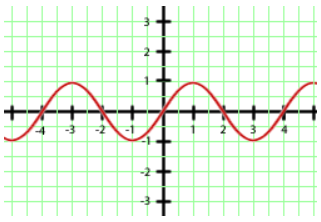
\includegraphics{samples/propiedades/periodicidad1.jpg}
	\end{figure}
	\begin{choices}
		\begin{choice}
			La función es periódica con periodo $T=2$.	
		\end{choice}
		\begin{choice}[x]
			La función es periódica con periodo $T=4$.
		\end{choice}	
		\begin{choice}
			La función no es periódica.
		\end{choice}
	\end{choices}
	\begin{feedback}
		Sus imágenes se repiten periódicamente en intervalos de longitud 4, por lo que la función es periódica con periodo $T=4$.
	\end{feedback}
\end{scq}

\vspace{1cm}


\begin{scq}
	Selecciona la opción correcta:\\
	\begin{figure}
		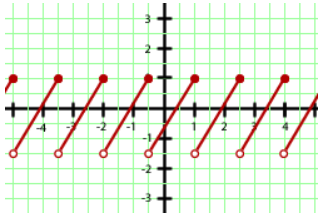
\includegraphics{samples/propiedades/periodicidad2.jpg}
	\end{figure}
	\begin{choices}
		\begin{choice}[x]s
			La función es periódica con periodo $T=2$.	
		\end{choice}
		\begin{choice}
			La función es periódica con periodo $T=4$.
		\end{choice}	
		\begin{choice}
			Ninguna de las respuestas anteriores es correcta.
		\end{choice}
	\end{choices}
	\begin{feedback}
		Sus imágenes se repiten periódicamente en intervalos de longitud 4, por lo que la función es periódica con periodo $T=2$.
	\end{feedback}
\end{scq}

\vspace{1cm}


\begin{scq}
	Selecciona la opción correcta:\\
	\begin{figure}
		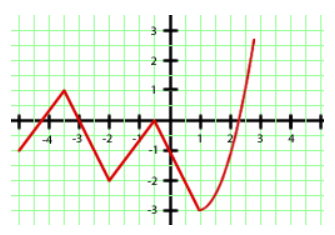
\includegraphics{samples/propiedades/periodicidad3.jpg}
	\end{figure}
	\begin{choices}
		\begin{choice}
			La función es periódica con periodo $T=5$.	
		\end{choice}
		\begin{choice}
			La función es periódica con periodo $T=6$.
		\end{choice}	
		\begin{choice}[x]
			La función no es periódica.
		\end{choice}
	\end{choices}
	\begin{feedback}
		No hay intervalos de igual longitud donde se repiten las imágenes, por lo que la función no es periódica.
	\end{feedback}
\end{scq}



\begin{scq}
	Selecciona la opción correcta:\\
	\begin{figure}
		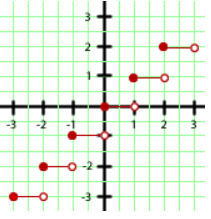
\includegraphics{samples/propiedades/periodicidad4.jpg}
	\end{figure}
	\begin{choices}
		\begin{choice}
			La función es periódica con periodo $T=1$.	
		\end{choice}
		\begin{choice}[x]
			La función es periódica con periodo $T=2$.
		\end{choice}	
		\begin{choice}[x]
			La función no es periódica.
		\end{choice}
	\end{choices}
	\begin{feedback}
		No hay intervalos de igual longitud donde se repiten las imágenes, por lo que la función no es periódica.
	\end{feedback}
\end{scq}



\begin{scq}
	Selecciona la opción correcta:\\
	\begin{figure}
		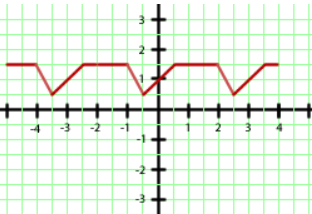
\includegraphics{samples/propiedades/periodicidad5.jpg}
	\end{figure}
	\begin{choices}
		\begin{choice}
			La función es periódica con periodo $T=-3$.	
		\end{choice}
		\begin{choice}[x]
			La función es periódica con periodo $T=3$.
		\end{choice}	
		\begin{choice}
			La función no es periódica.
		\end{choice}
	\end{choices}
	\begin{feedback}
		Sus imágenes se repiten periódicamente en intervalos de longitud 3, por lo que la función es periódica con periodo $T=3$.
	\end{feedback}
\end{scq}


\subsection{Puntos de corte con los ejes}

Si una función corta el \textbf{eje de abscisas}, lo hace en los puntos $(x, 0)$, es decir, los puntos donde $f(x)=0$.\\
\\
Si una función corta el \textbf{eje de ordenadas}, lo hace en el punto $(0, f(0))$, si $0$ pertenece al dominio de la función.\\
\\
Una función puede cortar el eje de abscisas varias veces, una vez o ninguna, pero no puede cortar el eje de ordenadas en más de un punto, dado que en dicho caso no sería una función.\\
\\
Para calcular los puntos de corte con el eje de abscisas, se debe de igualar la función a $0$. Siendo el valor obtenido el valor de la $x$ y el 0 el valor de la $y$. En el caso de los puntos de corte del eje de ordenadas, para calcular el valor de la $y$ correspondiente al punto que posee $x=0$, se debe de calcular el valor de la función en $0$, $y=f(0)$.\\
\youtube{FnauclNt3do}
\subsubsection{Signo de una función}
Determinar el signo de una función consiste en hallar las zonas donde la función está por encima o por debajo del eje de abscisas, es decir, los valores del dominio para los cuales $f(x) > 0$ o $f(x) < 0$ .\\
\\
Para determinar el signo de la función debemos representar en el eje de abscisas los puntos de corte de la función con dicho eje y los puntos donde la función no está definida. Después, analizamos el signo de la función en los distintos trozos.
\subsubsection{Ejercicios}

\begin{ex}[sol later]
	Determina los puntos de corte con los ejes de la función $f(x)=x^2$
	\begin{sol}
		El punto de corte con los ejes es: $(0,0)$
		\geogebra{un6xmbsf}
	\end{sol}
\end{ex}

\vspace{1cm}

\begin{ex}[sol later]
	Determina los puntos de corte con los ejes de la función $f(x)=\dfrac{3x^2}{x^2+1}$
	\begin{sol}
		El punto de corte con los ejes es: $(0,0)$
		\geogebra{fd2tfayt}
	\end{sol}
\end{ex}

\vspace{1cm}

\begin{ex}[sol later]
	Determina los puntos de corte con los ejes de la función $f(x)=x^4-2x^2$
	\begin{sol}
		Los puntos de corte con los ejes son $(0,0), (\sqrt{2}, 0)$ y $(-\sqrt{2}, 0)$
		\geogebra{e4fb746d}
	\end{sol}
\end{ex}

\vspace{1cm}

\begin{ex}[sol later]
	Determina los puntos de corte con los ejes de la función $f(x)=\sqrt{x^2-1}$
	\begin{sol}
		Los puntos de corte con los ejes son $(1, 0)$ y $(-1, 0)$
		\geogebra{mrr3hqe8}
	\end{sol}
\end{ex}

\vspace{1cm}

\begin{ex}[sol later]
	Determina los puntos de corte con los ejes de la función $f(x)=\dfrac{1}{x^2-9}$
	\begin{sol}
		El punto de corte con los ejes es: $(0,-\dfrac{1}{9})$
		\geogebra{cfme2yq3}
	\end{sol}
\end{ex}

\vspace{1cm}





\begin{ex}[sol later]
	Determina los puntos de corte con los ejes de la función que se muestra a continuación:\\
	\geogebra{mvmuqk5u}
	\begin{sol}
		El punto de corte con los ejes es: $(0,1)$
	\end{sol}
\end{ex}

\vspace{1cm}

\begin{ex}[sol later]
	Determina los puntos de corte con los ejes de la función que se muestra a continuación:\\
	\geogebra{d4audnb2}
	\begin{sol}
		No hay puntos de corte con los ejes.
	\end{sol}
\end{ex}

\vspace{1cm}

\begin{ex}[sol later]
	Determina los puntos de corte con los ejes de la función que se muestra a continuación:\\
	\geogebra{mv8baxdm}
	\begin{sol}
		No hay puntos de corte con los ejes.
	\end{sol}
\end{ex}

\vspace{1cm}

\begin{ex}[sol later]
	Determina los puntos de corte con los ejes de la función que se muestra a continuación:\\
	\geogebra{kcbmtz7k}
	\begin{sol}
		El punto de corte con los ejes es: $(0,0)$
	\end{sol}
\end{ex}

\vspace{1cm}

\begin{ex}[sol later]
	Determina los puntos de corte con los ejes de la función que se muestra a continuación:\\
	\geogebra{fw3xywww}
	\begin{sol}
		El punto de corte con los ejes es: $(0,0)$
	\end{sol}
\end{ex}


\subsection{Continuidad}


Intuitivamente, una función es \textbf{continua} si su gráfica se puede trazar sin levantar el lápiz del papel.\\
\\
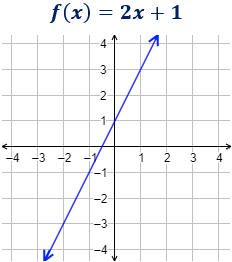
\includegraphics{samples/propiedades/funcionContinua.jpg}\\

Cuendo existen puntos en los que es necesario levantar el lápiz del papel, se dice que la función es \textbf{discontinua} en estos puntos, que se denominan \textbf{puntos de discontinuidad}.\\
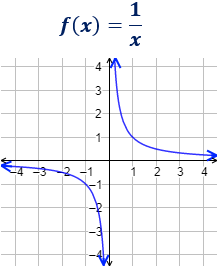
\includegraphics{samples/propiedades/funcionDiscontinua.jpg}

\subsubsection{Ejercicios}
\begin{ex}[sol later]
	Estudia la continuidad de las siguientes funciones::\\
	\begin{itemize}
		\item $f(x) = \dfrac{1}{x-2}$
		\item $f(x) = \dfrac{1}{3x^2-27}$
		\item $f(x) = \dfrac{x^2-2x}{2x^2+3x-2}$
		\item $f(x) = \sqrt{x^2+2x+1}$
		\item $f(x) = \sqrt{3x^2-3x-6}$
		\item $f(x) = \dfrac{\sqrt{x^2-1}}{x^4-x^3-x^2+x}$
		\item $f(x) = \dfrac{2x^2-x}{\sqrt{x^3+x^2-x-1}}$
		\item $f(x) = 3^{\dfrac{1}{x^2-1}}$
		\item $f(x) = \log(x^2-4x+4)$
	\end{itemize}
	\begin{sol}
		\begin{itemize}
			\item Dom(f) = $\mathbb{R}-\{2\}$. Función continua en todo su dominio.
			\item Dom(f) = $\mathbb{R}-\{-3,3\}$. Función continua en todo su dominio.
			\item Dom(f) = $\mathbb{R}-\{\dfrac{1}{2}\}$. Función continua en todo su dominio.
			\item Dom(f) = $\mathbb{R}$. Función continua en todo su dominio.
			\item Dom(f) = $(-\infty, -1] \bigcup [2,+\infty)$. Función continua en todo su dominio.
			\item Dom(f) = $\mathbb{R}-[-1,1]$. Función continua en todo su dominio.
			\item Dom(f) = $[1,+\infty)$. Función continua en todo su dominio.
			\item Dom(f) = $\mathbb{R}-\{-1, 1\}$. Función continua en todo su dominio.
			\item Dom(f) = $\mathbb{R}-\{2\}$. Función continua en todo su dominio.
		\end{itemize}
	\end{sol}
\end{ex}


\subsection{Crecimiento y decrecimiento}
\begin{definition}
	Una función $f$ es \textbf{creciente} en un intervalo si para cualesquiera $x_1$ y $x_2$ del intervalo tales que $x_{1} < x_{2}$, se verifica que $f(x_{1}) \leq f(x_{2})$.
\end{definition}
Si la desigualdad es estricta, es decir, si para cualesquiera $x_1$ y $x_2$ tales que $x_1 < x_2$ se verifica que $f(x_{1}) < f(x_{2})$, la función es \textbf{estrictamente creciente}.\\
\newline
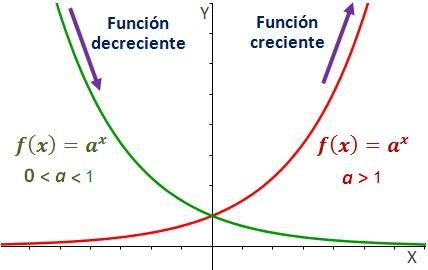
\includegraphics{samples/propiedades/crecienteDecreciente.jpg}\\
\begin{definition}
	Una función $f$ es \textbf{decreciente} en un intervalo si para cualesquiera $x_1$ y $x_2$ del intervalo tales que $x_{1} < x_{2}$, se verifica que $f(x_{1}) \geq f(x_{2})$.	
\end{definition}
Como en el caso anterior, si para cualesquiera $x_1$ y $x_2$ tales que $x_{1} < x_{2}$ se verifica que $f(x_{1}) > f(x_{2})$, la función es \textbf{estrictamente decreciente}.\\
\youtube{cWqJfem3GTk}
\subsubsection{Ejercicios}

\begin{ex}[sol later]
	Determina los intervalos de crecimiento y decrecimiento de la función $f(x)=x^4-2x^2-8$
	\begin{sol}
		\begin{itemize}
			\item Crecimiento: $(-1,0) \bigcup (1,+\infty)$
			\item Decrecimiento: $(-\infty, -1) \bigcup (0,1)$
		\end{itemize}
		\geogebra{rahsjufx}
	\end{sol}
\end{ex}

\vspace{1cm}

\begin{ex}[sol later]
	Determina los intervalos de crecimiento y decrecimiento de la función $f(x)=3x^4-20x^3-6x^2+60x-8$
	\begin{sol}
		\begin{itemize}
			\item Crecimiento: $(-1,1) \bigcup (5, +\infty)$
			\item Decrecimiento: $(-\infty, -1) \bigcup (1,5)$
		\end{itemize}
		\geogebra{z2jageyv}
	\end{sol}
\end{ex}

\vspace{1cm}

\begin{ex}[sol later]
	Determina los intervalos de crecimiento y decrecimiento de la función $f(x)=\dfrac{x+1}{x^2+x-2}$
	\begin{sol}
		\begin{itemize}
			\item Decrecimiento: $\mathbb{R}-\{-2,1\}$ 
		\end{itemize}
		\geogebra{zjmqndnw}
	\end{sol}
\end{ex}

\vspace{1cm}

\begin{ex}[sol later]
	Determina los intervalos de crecimiento y decrecimiento de la función $f(x)=\dfrac{x^4+1}{x^2}$
	\begin{sol}
		\begin{itemize}
			\item Crecimiento: $(-1,0) \bigcup (1, +\infty)$
			\item Decrecimiento: $(-\infty, -1) \bigcup (0,1)$ 
		\end{itemize}
		\geogebra{ct2hh9nx}
	\end{sol}
\end{ex}

\vspace{1cm}

\begin{ex}[sol later]
	Determina los intervalos de crecimiento y decrecimiento de la función $f(x)=\dfrac{x}{1+x^2}$
	\begin{sol}
		\begin{itemize}
			\item Crecimiento: $(-1,1)$
			\item Decrecimiento: $(-\infty, -1) \bigcup (1, +\infty)$ 
		\end{itemize}
		\geogebra{m6jd6rcj}
	\end{sol}
\end{ex}

\vspace{1cm}

\begin{ex}[sol later]
	Trata de observar los intervalos de crecimiento y de crecimiento de las siguientes funciones ayudándote de la representación gráfica de las mismas:
	\begin{itemize}
		\item $f(x) = x + \sqrt{x}$
		\item $f(x) = e^{\dfrac{1}{x}}$
		\item $f(x) = (x-1)e^{-x}$
		\item $f(x) = \dfrac{\ln(x)}{x}$
	\end{itemize}
	\geogebra[stb=true, ai=true]{tc5pbmae}
	\begin{sol}
		Juega con el applet de Geogebra.
	\end{sol}
\end{ex}


\subsection{Máximos y mínimos relativos y absolutos}
\begin{definition}
	Una función tiene un \textbf{máximo relativo} en $x=a$ si para todo $x$ de un entorno de $a$ se verifica que $f(a)$ es mayor o igual que $f(x)$.
\end{definition}

\begin{definition}
	Una función tiene un \textbf{mínimo relativo} en $x=a$ si para todo $x$ de un entorno de $a$ se verifica que $f(a)$ es menor o igual que $f(x)$.
\end{definition}

\begin{definition}
	Una función tiene un \textbf{máximo(mínimo) absoluto} en $x=a$ si para todo $x$ ded $Dom (f)$ se verifica que $f(a)$ es mayor(menor) o igual que $f(x)$.
\end{definition}

En la siguiente función, se puede observar cuales son los máximos y los mínimos relativos.
\geogebra{bxmrfp5r}
\subsubsection{Ejercicios}
\begin{ex}[sol later]
	Clacula los máximos y los mínimos de las siguientes funciones:\\
	\begin{itemize}
		\item \geogebra{uxmbmw2k}
		\item \geogebra{mubhyvzv}
		\item \geogebra{whfwaz4t}
	\end{itemize}
	\begin{sol}
		\begin{itemize}
			\item Máximo: $(0,0)$
			\item No presenta ni máximos ni mínimos.
			\item Máximo: $(1,3)$ \\ Mínimo: $(3,-1)$
		\end{itemize}
	\end{sol}
\end{ex}

\vspace{1cm}

\begin{ex}[sol later]
	Calcula los máximos y los mínimos de las siguientes funciones:\\
	\begin{itemize}
		\item $f(x)=x^3-3x^2+3$
		\geogebra{kesnfpdm}
		\item $f(x)=3x^4-4x^3$
		\geogebra{v7cynn2w}
		\item $f(x)=\dfrac{3}{x^2+1}$
		\geogebra{g6kcsfkb}
	\end{itemize}
	\begin{sol}
		\begin{itemize}
			\item Máximo en $x=0$ y mínimo en $x=2$.
			\item Mínimo en $x=1$.
			\item Máximo en $x=0$.
		\end{itemize}
	\end{sol}
\end{ex}


\subsection{Concavidad y puntos de inflexión}
\begin{definition}
Un \textbf{punto de inflexión} de una función es un punto en el que la función cambia de convexa $(\bigcup)$ a cóncava $(\bigcap)$, o viceversa, y la tangente atraviesa la gráfica.
\end{definition}
A continuación se muestra un ejemplo de punto de inflexión.
\geogebra{kzzn4gj2}


\begin{definition}
Estudiar la \textbf{curvatura} de una función consiste en estudiar en qué intervalos es convexa $(\bigcup)$ y en cuáles es cóncava $(\bigcap)$. Los intervalos de curvatura están separados por los puntos de inflexión y las discontinuidades.
\end{definition}

\subsubsection{Ejercicios}
\begin{ex}[sol later]
	Calcula los puntos de inflexión de las siguientes funciones:\\
	\begin{itemize}
		\item $f(x)=-x^3+3x$
		\geogebra{tkhxm6jf}
	\end{itemize}
	\begin{sol}
		\begin{itemize}
			\item Punto de inflexión en $(0,0)$.
		\end{itemize}
	\end{sol}
\end{ex}





\section{Análisis gráficos de funciones}
Documento basado en muestra proporcionada por Prof. Toby Roberts (disponible \href{http://www.maths.adelaide.edu.au/anthony.roberts/LaTeX/Src/maths.tex}{aquí}).

\subsection{Análisis de la gráfica}
Hacer el estudio sobre una gráfica de una función consiste en analizar sus características a partir de lo que se observa en la gráfica. Para realizar este estudio, es necesario llevar a cabo, ordenadamente, los pasos que se indican en la siguiente tabla.\\
\begin{table}[]
	
	\begin{tabular}{|p{5cm}|}
		\hline
		\textbf{Formulario: características}\\ \hline
		\textbf{1. Tipo de función:} consiste en clasificar la función. \\ \hline
		\textbf{2. Dominio de una función:} conjunto de valores que toma la variable inependiente \textbf{x}. Se representa por \textbf{Dom(f)}.\\ \hline
		\textbf{3. Periodicidad de una función:} una función es periódica si se repite en intervalos iguales.\\ \hline
		\textbf{4. Simetría de una función:} se estudiarán sólo las simetrías respecto del origen O(0,0) y respecto del eje Y.\\ \hline
		\textbf{5. Asíntotas de una función:} rectas a las que se acerca la función en puntos muy alejados del origen sin llegar a tocarlas. Las asíntotas pueden ser verticales, horizontales y oblicuas. \\ \hline
		\textbf{6. Puntos de corte de una función con los ejes:} puntos en que $x=0$ y/o $y=0$. La gráfica puede cortar al eje X en varios puntos; al eje Y, como máximo, en uno.\newline \textbf{Signo:} intervalos del eje X en los que la función es positiva (+) o negativa (-). Las regiones están separadas por las abscisas de los puntos de corte del eje X y por las discontinuidades. \\ \hline
		\textbf{7. Máximos y mínimos relativos de una función:}\newline \textbf{Máximo relativo:} punto en el que el valor de la función es mayor que en los puntos que están muy cercanos.\newline \textbf{Mínimo relativo: } punto en que el valor de la función es menor que en los puntos que están muy cercanos.\newline \textbf{Monotonía: } consiste en estudiar en qué intervalos la función es creciente y en cuáles es decreciente. Los intervalos de crecimiento están separados por las abscisas de los máximos y mínimos relativos y por las discontinuidades. \\ \hline
		\textbf{8. Punto de inflexión de una función:} punto en que la función cambia de convexa $(\bigcup)$ a cóncava $(\bigcap)$ o viceversa, es decir, la recta tangente atraviesa a la gráfica.\newline \textbf{Curvatura:} consiste en estudiar en qué intervalos es convexa $(\bigcup)$ y en cuáles es cóncava $(\bigcap)$. Los intervalos de curvatura están separados por las abscisas de los puntos de inflexión y las discontinuidades.\\ \hline
		\textbf{9. Recorrido o imagen de una función:} conjunto de valores que toma la variable dependiente \textbf{y}. Se representa por \textbf{Im(f)}.\\ \hline
	\end{tabular}
	
\end{table}



\subsection{Clasificación de funciones}
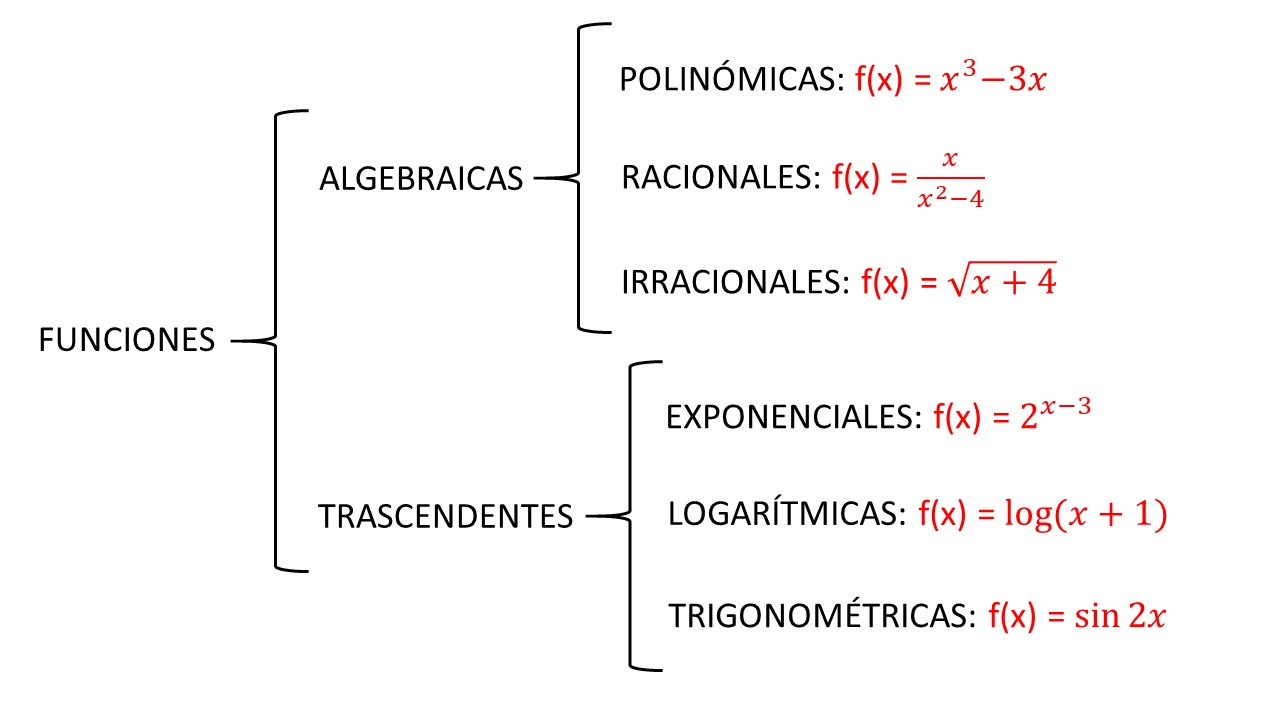
\includegraphics{samples/analisis/clasificaEsquema2.jpg}
\subsubsection{Ejemplos}
\begin{itemize}
	\item \textbf{Polinómicas.}
	$f(x) = x^3-3x$
	\geogebra{cwt7r5f7}
	\item \textbf{Racionales.}
	$f(x) = \dfrac{x}{x^2-4}$
	\geogebra{cdwjf88d}
	\item \textbf{Irracionales.}
	$f(x) = \sqrt{x+4}$
	\geogebra{xjn6vrn8}
	\item \textbf{Exponenciales.}
	$f(x) = 2^{x-3}$
	\geogebra{faj4urcm}
	\item \textbf{Logarítmicas.}
	$f(x) = \ln (x-1)$
	\geogebra{apzz89ae}
	\item \textbf{Trigonométricas.}
	$f(x) = \sin(2x)$
	\geogebra{yvw8jubg}
\end{itemize}

\subsection{Funciones polinómicas}
\youtube{YXUf8a3M9vk}
\subsubsection{Modelo de función polinómica}
Analiza y representa la función $y = 2x^2 - \dfrac{x^4}{4}$
\begin{itemize}
	\item \textbf{1. Tipo de función: }polinómica.
	\item \textbf{2. Dominio: }por ser una función polinómica, es toda la recta real $\mathbb{R}$ \\
	Dom(f) = $\mathbb{R} = (-\infty, +\infty)$.
	\item \textbf{3. Continuidad: }por ser polinómica, es toda la recta real $\mathbb{R}$.
	\item \textbf{4. Periodicidad: }no es periódica porque las funciones polinómicas nunca lo son.
	\item \textbf{5. Simetrías: }$f(-x)=2(-x)^2-\dfrac{(-x)^4}{4}=2x^2-\dfrac{x^4}{4}$\\ Se observa que $f(-x)=f(x) \rightarrow$ función par $\rightarrow$ simetría respecto del eje Y.
	\item \textbf{6. Asíntotas: }las funciones polinómicas no tienen asíntotas.
	\item \textbf{7. Corte con los ejes.}
	\begin{itemize}
	\item \textbf{Eje X: }$2x^2-\dfrac{x^4}{4}=0 \rightarrow x=0$, raíz doble; $x_1=2\sqrt{2}$, $x_2=-2\sqrt{2}$, raíces simples.\\
	Se obtienen los puntos $O(0,0)$, $A(-2\sqrt{2},0)$, $B(2\sqrt{2},0)$
	\item \textbf{Eje Y: }es el punto $O(0,0)$
	\item \textbf{Signo: }Si $x=1 \rightarrow f(1)=2-\dfrac{1}{4}=\dfrac{7}{4}>0$ (+)
	\end{itemize}
	\item \textbf{8. Máximos y mínimos:}\\
		$f'(x)=4x-x^3 \rightarrow 4x-x^3=0 \rightarrow x_1 = 0, x_2 = -2, x_3=2$, raíces simples.\\
		$f(x)=2x^2-\dfrac{x^4}{4}$\\
		\begin{itemize}
			\item $f(-2)=4 \rightarrow C(-2,4$)\\
			\item $f(0)=0 \rightarrow O(0,0)$\\
			\item $f(2)=4 \rightarrow D(2,4)$\\
		\end{itemize}
		$f''(x)=4-3x^2$
		\begin{itemize}
			\item $f''(-2)=-8 <0 \rightarrow C(-2,4)$ \textbf{máximo relativo}.\\
			\item $f''(0)=4 >0 \rightarrow O(0,0)$ \textbf{mínimo relativo}.\\
			\item $f''(2)=-8 <0 \rightarrow D(2,4)$ \textbf{máximo relativo}.\\
		\end{itemize}
		\textbf{Monotonía:}\\
		$f'(x)=4x-x^3 \rightarrow$ Si $x=1 \rightarrow f'(x)=4-1=3 > 0$ (+)
	\item \textbf{9. Puntos de inflexión:}\\
	$f''(x)= 4-3x^2 \rightarrow 4-3x^2=0 \rightarrow x_1= -\dfrac{2\sqrt{3}}{3}$, $x_2=\dfrac{2\sqrt{3}}{3}$ raíces simples.\\
	$f(x) = 2x^2-\dfrac{x^4}{4}$
	\begin{itemize}
		\item $f(-\dfrac{2\sqrt{3}}{3}) = \dfrac{20}{9} \rightarrow E(-\dfrac{2\sqrt{3}}{3}, \dfrac{20}{9})$
		\item $f(\dfrac{2\sqrt{3}}{3}) = \dfrac{20}{9} \rightarrow F(\dfrac{2\sqrt{3}}{3}, \dfrac{20}{9})$
	\end{itemize}
	$f'''(x)=-6x$
	\begin{itemize}
		\item $f'''(-\dfrac{2\sqrt{3}}{3}) = 4\sqrt{3} \neq 0 \rightarrow E(-\dfrac{2\sqrt{3}}{3}, \dfrac{20}{9})$, \textbf{punto de inflexión}.
		\item $f'''(\dfrac{2\sqrt{3}}{3}) = -4\sqrt{3} \neq 0 \rightarrow F(\dfrac{2\sqrt{3}}{3}, \dfrac{20}{9})$, \textbf{punto de inflexión}.
	\end{itemize}
	\item \textbf{10. Curvatura:}\\
	$f''(x)=4-3x^2 \rightarrow$ Si $x=0 \rightarrow f''(0)=4 > 0$ (+)
\end{itemize}
\geogebra{ceu6sks6}


\subsection{Funciones racionales}
\youtube{ARUEwJ_7sGc}
\subsubsection{Modelo de función racional}
Analiza y representa la función $y=\dfrac{x^3}{x^2-1}$
\begin{itemize}
	\item \textbf{1. Tipo de función: }racional.
	\item \textbf{2. Dominio: }por ser una función racional, hay que excluir las raíces del denominador: $x^2-1=0 \rightarrow x^2=1 \rightarrow x_1=-1$, $x_2=1$.\\
	$Dom(f) = \mathbb{R}-\{-1,1\} = (-\infty, -1) \bigcup (-1,1) \bigcup (1,+\infty)$
	\item \textbf{3. Continuidad: }es discontinua en $x=-1$, $x=1$, donde presenta discontinuidades de 1ª especie de salto finito.
	\item \textbf{4. Periodicidad: }no es periódica porque las funciones racionales nunca lo son.
	\item \textbf{5. Simetrías: }$f(-x)=\dfrac{(-x)^3}{(-x)^2-1}=\dfrac{-x^3}{x^2-1}=-\dfrac{x^3}{x^2-1}$\\
	Se observa que $f(-x) = -f(x) \rightarrow$ función impar $\rightarrow$ simetría respecto al origen $O(0,0)$
	\item \textbf{6. Asíntotas: }
	\begin{itemize}
		\item Verticales: son las raíces del denominador, $x=-1$, $x=1$\\
		Posición de la curva respecto a las asíntotas verticales:\\
		$$\lim_{x \to -1^{-}}(\dfrac{x^3}{x^2-1})=\dfrac{(-1^{-})^3}{(-1^{-})^2-1}=\dfrac{-1}{0^{+}}=-\infty$$
		$$\lim_{x \to -1^{+}}(\dfrac{x^3}{x^2-1})=\dfrac{(-1^{+})^3}{(-1^{+})^2-1}=\dfrac{-1}{0^{-}}=+\infty$$
		$$\lim_{x \to 1^{-}}(\dfrac{x^3}{x^2-1})=\dfrac{(1^{-})^3}{(1^{-})^2-1}=\dfrac{1}{0^{-}}=-\infty$$
		$$\lim_{x \to 1^{+}}(\dfrac{x^3}{x^2-1})=\dfrac{(1^{+})^3}{(1^{+})^2-1}=\dfrac{1}{0^{+}}=+\infty$$
		\item Horizontales: no tiene.
		\item Oblicuas: $y=x$\\
		Posición de la curva respecto de la asíntota oblicua:
		$$\lim_{x \to -\infty}(\dfrac{x}{x^2-1})=\dfrac{-\infty}{(-\infty)^2-1}=0^{-}$$
		$$\lim_{x \to +\infty}(\dfrac{x}{x^2-1})=\dfrac{+\infty}{(+\infty)^2-1}=0^{+}$$
	\end{itemize}
	\item \textbf{7. Corte con los ejes:}
	\begin{itemize}
		\item \textbf{Eje X: }$x^3=0 \rightarrow x=0$ raíz triple. Se obtiene el punto $O(0,0)$.
		\item \textbf{Eje Y: }el punto $O(0,0)$.
		\item \textbf{Signo: }Si $x=2 \rightarrow f(2)=\dfrac{2^3}{2^2-1}=\dfrac{8}{3}>0$(+)
	\end{itemize}
	\item \textbf{8. Máximos y mínimos relativos:}\\
	$x^2(x^2-3)=0 \rightarrow x=0 $raíz doble; $x=-\sqrt{3}$, $x=\sqrt{3}$ raíces simples.\\
	$f''(-\sqrt{3})=-\dfrac{3\sqrt{3}}{2}<0 \rightarrow A(-\sqrt{3}, -\dfrac{3\sqrt{3}}{2})$, \textbf{máximo relativo}.\\
	$f''(\sqrt{3})=\dfrac{3\sqrt{3}}{2}>0 \rightarrow B(\sqrt{3}, \dfrac{3\sqrt{3}}{2})$, \textbf{mínimo relativo}.\\
	\textbf{Monotonía: }\\
	$f'(x)=\dfrac{x^4-3x^2}{(x^2-1)^2} \rightarrow$ Si $x=2 \rightarrow f'(2)=\dfrac{2^4-3 \cdot 2^2}{(2^2-1)^2}=\dfrac{4}{9}>0$(+)\\
	Las raíces del denominador son discontinuidades dobles.
	\item \textbf{9. Puntos de inflexión:}\\
	$2x(x^2+3) = 0 \rightarrow x=0$ raíz simple.\\
	$f'''(x) = - \dfrac{6x^4+36x^2+6}{(x^2-1)^4} \rightarrow f'''(0)=-6 \neq 0 \rightarrow O(0,0)$, \textbf{punto de inflexión}.\\
	\textbf{Curvatura:}\\
	$f''(x)=\dfrac{2x^3+6x}{(x^2-1)^3} \rightarrow$ Si $x=2 \rightarrow f''(2)=\dfrac{2 \cdot 2^3+6 \cdot 6}{(2^2-1)^3}=\dfrac{28}{27}>0$(+)\\
	Las raíces del denominador son discontinuidades triples.
	
\end{itemize}
\geogebra{s2j8hxtz}

\subsection{Funciones irracionales}
\youtube{akSVuDk_lhw}
\subsubsection{Modelo de función irracional}
Analiza y representa la función $y=\sqrt{x^2-4}$
\begin{itemize}
	\item \textbf{1. Tipo de función: }irracional.
	\item \textbf{2. Dominio: }por ser una función irracional de índice par, el radicando tiene que ser mayor o igual que cero.\\
	$x^2-4 \geq 0$, se resuelve la ecuación correspondiente $x^2-4=0 \rightarrow x^2=4 \rightarrow x_1=-2$, $x_2=2$. Como las raíces son simples, $x^2-4$ cambia de signo en cada una de ellas.\\
	Dom(f)= $(-\infty, -2] \bigcup [2, +\infty)$
	\item \textbf{3. Continuidad: }es discontinua en $x=-2$, $x=2$.
	\begin{itemize}
		\item Para $x=-2$, se tiene $f(-2)=0$:
		$$\lim_{x \to -2^{-}}(\sqrt{x^2-4})=0$$
		$$\lim_{x \to -2^{+}}(\sqrt{x^2-4}) \text{no existe}$$
		Por tanto, para $x=-2$, la función tiene una discontinuidad de 2ª especie.\\
		\item Para $x=-2$, se tiene $f(-2)=0$:
		$$\lim_{x \to 2^{-}}(\sqrt{x^2-4}) \text{no existe}$$
		$$\lim_{x \to 2^{+}}(\sqrt{x^2-4})=0$$
		Por tanto, para $x=2$, la función tiene una discontinuidad de 2ª especie.\\
	\end{itemize}
	\item \textbf{4. Periodicidad: }no es periódica. Las funciones irracionales nunca lo son.
	\item \textbf{5. Simetrías: }$f(-x) = \sqrt{(-x)^2-4} = \sqrt{x^2-4}$\\
	Se observa que $f(-x)=f(x) \rightarrow $función par $\rightarrow$ simétrica respecto al eje Y.
	\item \textbf{6. Asíntotas: }
	\begin{itemize}
		\item Verticales: no tiene.
		\item Horizontales: no tiene.
		\item Oblicuas: presenta asíntotas oblicuas en $y=x$ y en $y=-x$.
	\end{itemize}
	\item \textbf{7. Corte con los ejes: }
	\begin{itemize}
		\item \textbf{Eje X: }$\sqrt{x^2-4} = 0 \rightarrow x^2-4=0 \rightarrow x^2=4 \rightarrow x_1=-2$, $x_2=2$\\
		Se obtienen los puntos $A(-2, 0)$ y $B(2,0)$
		\item \textbf{Eje Y: }no lo corta.
		\item \textbf{Signo: }Si $x=3 \rightarrow f(3)=\sqrt{3^2-4}=\sqrt{9-4}=\sqrt{5}>0$ (+)
	\end{itemize}
	\item \textbf{8. Máximos y mínimos relativos: }
	$f'(x)=\dfrac{x}{\sqrt{x^2-4}} \rightarrow x=0 \notin$ Dom(f)\\
	No tiene ni máximos ni mínimos relativos.\\
	\textbf{Monotonía: }si $x=3 \rightarrow f'(3)=\dfrac{3}{\sqrt{3^2-4}}=\dfrac{3}{\sqrt{5}}>0$ (+)
	\item \textbf{9. Puntos de inflexión: }\\
	$f''(x)=-\dfrac{4}{(x^2-4)\sqrt{x^2-4}}$ \\
	$f''(x)$ nunca se hace cero, por lo tanto no ha puntos de inflexión.\\
	\textbf{Curvatura: }si $x=3 \rightarrow f''(3)=-\dfrac{4}{(3^2-4)\sqrt{3^2-4}}=-\dfrac{4}{5\sqrt{5}}<0$ (-)	
\end{itemize}
\geogebra{nxe84yaw}

\subsection{Funciones exponenciales}
\youtube{JulYyOS0hH4}
\subsubsection{Modelo de función exponencial}
Analiza y representa la función $y=(2-x)e^x$
\begin{itemize}
	\item \textbf{1. Tipo de función: }producto de polinómica por exponencial.
	\item \textbf{2. Dominio: }por ser el producto de una función polinómica por una función exponencial, es toda la recta real $\mathbb{R}$.\\
	Dom(f) = $\mathbb{R}=(-\infty, +\infty)$
	\item \textbf{3. Continuidad: }por ser el producto de una función polinómica por una exponencial, es continua en toda la recta real $\mathbb{R}$. 
	\item \textbf{4. Periodicidad: }no es periódica, ya que las funciones polinómicas y exponenciales nunca lo son.
	\item \textbf{5. Simetrías: }$f(-x)=(2+x)e^{-x}$\\
	Se observa que $f(-x)\neq f(x)$, $f(-x) \neq -f(x) \rightarrow$ no es simétrica ni respecto al eje Y ni respecto del orien $O(0,0)$.
	\item \textbf{6. Asíntotas: }\\
	\begin{itemize}
		\item Verticales: no tiene.
		\item Horizontales: \\
		$$\lim_{x \to -\infty}((2-x)e^x)=0$$
		$$\lim_{x \to +\infty}((2-x)e^x)=-\infty$$
		Asíntota horizontal $y=0$, pero sólo por la izquierda.\\
		Posición de la curva respecto de la asíntota oblicua:
		$$\lim_{x \to -\infty}((2-x)e^x)=0^{+}$$
		La curva está encima de la asíntota.
		\item Oblicuas: no tiene.
	\end{itemize}
	\item \textbf{7. Corte con los ejes: }
	\begin{itemize}
		\item \textbf{Eje X: }$(2-x)e^{x} = 0 \rightarrow x=2$, raíz simple. Se obtiene el punto $A(2,0)$.
		\item \textbf{Eje Y: }es el punto $B(0,2)$.
		\item \textbf{Signo: }Si $x=0 \rightarrow f(0)=2 >0$ (+)
	\end{itemize}
	\item \textbf{8. Máximos y mínimos relativos: }\\
	$f'(x)=(1-x)e^x \rightarrow (1-x)e^x = 0 \rightarrow x=1$, raíz simple.\\
	$f(x)=(2-x)e^x \rightarrow f(1)=e \rightarrow C(1,e)$\\
	$f''(x)=-ze^{x} \rightarrow f''(x)=-e < 0 \rightarrow C(1,e)$, \textbf{máximo relativo}.\\
	\textbf{Monotonía: }\\
	$f''(x)=(1-x)e^x \rightarrow $Si $x=0 \rightarrow f'(0) = 1>0$ (+) 
	\item \textbf{9. Puntos de inflexión:}\\
	$f''(x)=-xe^x \rightarrow -xe^x = 0 \rightarrow x=0$, raíz simple.\\
	$f(x)=(2-x)e^x \rightarrow f(0)=2 \rightarrow B(0,2)$\\
	$f'''(x)=-(x+1)e^x \rightarrow f'''(0)=-1 \neq 0 \rightarrow B(0,2)$, \textbf{punto de inflexión}.\\
	\textbf{Curvatura:}\\
	$f''(x)=-xe^x \rightarrow $si $x=1 \rightarrow f''(1)=-e<0$ (-)
	
\end{itemize}
\geogebra{cthuzvhc}

\subsection{Funciones logarítmicas}
\youtube{a7mRvMyayVM}
\subsubsection{Modelo de función logarítmica}
Analiza y representa la función $y=\ln (x^2-1)$
\begin{itemize}
	\item \textbf{1. Tipo de función: }logarítmica.
	\item \textbf{2. Dominio: }por ser una función logarítmica, el argumento tiene que ser positivo, es decir, mayor que cero.\\
	$x^2-1 >0$, se resuelve la ecuación correspondiente $x^2-1 = 0 \rightarrow x^2=1 \rightarrow x_1=-1$, $x_2=1$. Como las raíces son simples, en cada una de ellas $x^2-1$ cambia el signo.\\
	$x^2-1 \rightarrow $Si $x=0 \rightarrow 0^2-1 = -1 <0$ (-)\\
	Dom(f)=$(-\infty , -1)\bigcup(1, +\infty)$
	\item \textbf{3. Continuidad: }es discontinua en $x=-1, x=1$
	\begin{itemize}
		\item Para $x=-1$, se tiene $f(-1)$ no existe:\\
		$$\lim_{x \to -1^{-}}(\ln (x^2-1))=-\infty$$
		$$\lim_{x \to -1^{+}}(\ln (x^2-1)) \text{no existe}$$
		Por tanto, para $x=-1$, la función tiene una discontinuidad de 2ª especie.
		\item Para $x=1$, se tiene $f(1)$ no existe:\\
		$$\lim_{x \to 1^{-}}(\ln (x^2-1)) \text{no existe}$$
		$$\lim_{x \to 1^{+}}(\ln (x^2-1))=-\infty$$
		Por tanto, para $x=1$, la función tiene una discontinuidad de 2ª especie.
	\end{itemize}
	\item \textbf{4. Periodicidad: }no es periódica, porque las funciones logarítmicas nunca lo son.
	\item \textbf{5. Simetrías: }$f(-x)= \ln[(-x)^2-1] = \ln(x^2-1)$\\
	Se observa que $f(-x)=f(x) \rightarrow$ función par $\rightarrow$ simetría respecto del eje Y.
	\item \textbf{6. Asíntotas: }
	\begin{itemize}
		\item Verticales: $x=-1, x=1$\\
		Posición de la curva respecto de las asíntotas verticales:
		$$\lim_{x \to -1^{-}}(\ln (x^2-1))=-\infty$$
		$$\lim_{x \to -1^{+}}(\ln (x^2-1)) \text{no existe}$$
		$$\lim_{x \to 1^{-}}(\ln (x^2-1)) \text{no existe}$$
		$$\lim_{x \to 1^{+}}(\ln (x^2-1))=-\infty$$
		\item Horizontales: no tiene.
		\item Oblicuas: no tiene.
	\end{itemize}
	\item \textbf{7. Corte con los ejes: }
	\begin{itemize}
		\item \textbf{Eje X: }$\ln(x^2-1) = 0 \rightarrow x^2-1=1 \rightarrow x^2=2 \rightarrow x_1=-\sqrt{2}$, $x_2=\sqrt{2}$, raíces simples. Se obtienen los puntos $A(-\sqrt{2},0); B(\sqrt{2},0)$\\
		Se obtienen los puntos $A(-2, 0)$ y $B(2,0)$
		\item \textbf{Eje Y: }no lo corta.
		\item \textbf{Signo: }Si $x=2 \rightarrow f(2)=\ln(3)>0$ (+)
	\end{itemize}
	\item \textbf{8. Máximos y mínimos relativos: }\\
	$f'(x)=\dfrac{2x}{x^2-1} \rightarrow \dfrac{2x}{x^2-1} = 0 \rightarrow x=0 \notin$ Dom(f)\\
	No tiene ni máximos ni mínimos relativos.\\
	\textbf{Monotonía: }\\
	$f'(x) = \dfrac{2x}{x^2-1} \rightarrow $Si $x=2 \rightarrow f'(2)=\dfrac{2\cdot 2}{2^2-1} = \dfrac{4}{3}>0$ (+)
	\item \textbf{9. Puntos de inflexión: }\\
	$f''(x)=-\dfrac{2x^2+2}{(x^2-1)^{2}}$ \\
	$f''(x)$ nunca se hace cero, por lo tanto no ha puntos de inflexión.\\
	\textbf{Curvatura: }\\
	$f''(x)=-\dfrac{2x^2+2}{(x^2-1)^{2}}$ siempre es negativo $\rightarrow$ siempre es cóncava $(\bigcap)$.	
\end{itemize}
\geogebra{pgghxa8t}

\subsection{Funciones trigonométricas}
\subsubsection{Modelo de función trigonométrica}
Analiza y representa la función $y=3 \sin 2x$
\begin{itemize}
	\item \textbf{1. Tipo de función: }trigonométrica.
	\item \textbf{2. Dominio: }las funciones seno y coseno están definidas en todos los números reales $\mathbb{R}$.\\
	Dom(f) = $\mathbb{R}=(-\infty, +\infty)$
	\item \textbf{3. Periodicidad: }es periódica en, de período $\dfrac{2\pi}{2} = \pi$\\
	Solo la estudiaremos en el primer período positivo $[0, \pi)$
	\item \textbf{4. Simetrías: }$f(-x) = 3 \sin (-2x) = -3 \sin (2x)$\\
	Se observa que $f(-x)=-f(x) \rightarrow$ función impar $\rightarrow$ simétrica respecto al origen de coordenadas $O(0,0)$.
	\item \textbf{5. Asíntotas: }
	\begin{itemize}
		\item Verticales: no tiene.
		\item Horizontales: no tiene.
		\item Oblicuas: no tiene.
	\end{itemize}
	\item \textbf{6. Corte con los ejes: }
	\begin{itemize}
		\item \textbf{Eje X: }$3\sin(2x)=0 \rightarrow \sin(2x) = 0 \rightarrow x_1=0$, $x_2=\dfrac{\pi}{2}$, raíces simples; Se obtienen los puntos $O(0,0); A(\dfrac{\pi}{2}, 0)$.\\
		\item \textbf{Eje Y: }es el punto $O(0,0)$
		\item \textbf{Signo: }Si $x=\dfrac{\pi}{4} \rightarrow f(\dfrac{\pi}{4})=3\cdot \sin(\dfrac{2\pi}{4}) = 3 \sin(\dfrac{\pi}{2})>0$ (+)
	\end{itemize}
	\item \textbf{7. Máximos y mínimos: }\\
	\begin{itemize}
		\item $B(\dfrac{\pi}{4}, 3)$, \textbf{máximo relativo}
		\item $C(\dfrac{3\pi}{4}, -3)$, \textbf{mínimo relativo}.
	\end{itemize}
	\textbf{Monotonía: }\\
	\begin{itemize}
		\item Creciente: $(0, \dfrac{\pi}{4}) \bigcup (\dfrac{3\pi}{4}, \pi))$
		\item Decreciente: $(\dfrac{\pi}{4}, \dfrac{3\pi}{4})$
	\end{itemize}
	\item \textbf{8. Puntos de inflexión:}\\
	\begin{itemize}
		\item $O(0,0)$, \textbf{punto de inflexión}.
		\item $A(\dfrac{\pi}{2},0)$, \textbf{punto de inflexión}.
	\end{itemize}
	\textbf{Curvatura: }\\
	\begin{itemize}
		\item Convexa $(\bigcup)$: $(\dfrac{\pi}{2}, \pi)$.
		\item Cóncava $(\bigcap)$: $(0, \dfrac{\pi}{2})$
	\end{itemize}
\end{itemize}
\geogebra{jufgczka}
\subsubsection{Ejercicios}
\begin{ex}[sol later]
	Ayudándote del panel, representa gráficamente las tres funciones trigonométricas más conocidas y observa las diferencias.
	\geogebra[ai=true, stb=true]{tc5pbmae}
	\begin{sol}
		Las funciones que se deben representar son el coseno, el seno y la tangente.
	\end{sol}
\end{ex}



\section{Matemáticas}

Documento basado en muestra proporcionada por Prof. Toby Roberts (disponible \href{http://www.maths.adelaide.edu.au/anthony.roberts/LaTeX/Src/maths.tex}{aquí}).

\subsection{Básicos}

\begin{itemize}
	\item Fórmulas delimitadas con dólares: $1<x<2$, $x^2+y^2=9$ y $y=\sqrt{9-x^2}$

	\item Fórmulas delimitadas con paréntesis: \(1\le x \le 2\), \(x^2+y^2=9\) y  \(y=\sqrt{9-x^2}\)
	
	\item Fórmula delimitada con doble dolar: 
	$$\int_a^b f(x)dx.$$
	
	\item Fórmula delimitada con corchetes: 
	\[\int_a^b f(x)dx.\]
\end{itemize}

\subsection{Delimiters}

See how the delimiters are of reasonable size in these examples
\[
	\left(a+b\right)\left[1-\frac{b}{a+b}\right]=a\,,
\]
\[
	\sqrt{|xy|}\leq\left|\frac{x+y}{2}\right|,
\]
even when there is no matching delimiter
\[
	\int_a^bu\frac{d^2v}{dx^2}\,dx
	=\left.u\frac{dv}{dx}\right|_a^b
	-\int_a^b\frac{du}{dx}\frac{dv}{dx}\,dx.
\]






\subsection{Spacing}

Differentials often need a bit of help with their spacing as in
\[
	\iint xy^2\,dx\,dy 
	=\frac{1}{6}x^2y^3,
\]
whereas vector problems often lead to statements such as
\[
	u=\frac{-y}{x^2+y^2}\,,\quad
	v=\frac{x}{x^2+y^2}\,,\quad\text{and}\quad
	w=0\,.
\]
Occasionally one gets horrible line breaks when using a list in mathematics such as listing the first twelve primes  \(2,3,5,7,11,13,17,19,23,29,31,37\)\,.
In such cases, perhaps include \verb|\mathcode`\,="213B| inside the inline maths environment so that the list breaks: \(\mathcode`\,="213B 2,3,5,7,11,13,17,19,23,29,31,37\)\,.
Be discerning about when to do this as the spacing is different.






\subsection{Arrays}

Arrays of mathematics are typeset using one of the matrix environments as 
in
\[
	\begin{bmatrix}
		1 & x & 0 \\
		0 & 1 & -1
	\end{bmatrix}\begin{bmatrix}
		1  \\
		y  \\
		1
	\end{bmatrix}
	=\begin{bmatrix}
		1+xy  \\
		y-1
	\end{bmatrix}.
\]
Case statements use cases:
\[
	|x|=\begin{cases}
		x, & \text{if }x\geq 0\,,  \\
		-x, & \text{if }x< 0\,.
	\end{cases}
\]
Many arrays have lots of dots all over the place as in
\[
	\begin{matrix}
		-2 & 1 & 0 & 0 & \cdots & 0  \\
		1 & -2 & 1 & 0 & \cdots & 0  \\
		0 & 1 & -2 & 1 & \cdots & 0  \\
		0 & 0 & 1 & -2 & \ddots & \vdots \\
		\vdots & \vdots & \vdots & \ddots & \ddots & 1  \\
		0 & 0 & 0 & \cdots & 1 & -2
	\end{matrix}
\]






\subsection{Equation arrays}

In the flow of a fluid film we may report
\begin{align}
	u_\alpha & =  \epsilon^2 \kappa_{xxx} 
	\left( y-\frac{1}{2}y^2 \right),
	\label{equ}  
	\\
	v & =  \epsilon^3 \kappa_{xxx} y\,,
	\label{eqv}  
	\\
	p & =  \epsilon \kappa_{xx}\,.
	\label{eqp}
\end{align}
Alternatively, the curl of a vector field $(u,v,w)$ may be written 
with only one equation number:
\begin{align}
	\omega_1 & = 
	\frac{\partial w}{\partial y}-\frac{\partial v}{\partial z}\,,
	\nonumber  \\
	\omega_2 & = 
	\frac{\partial u}{\partial z}-\frac{\partial w}{\partial x}\,,
	\label{eqcurl}  
	\\
	\omega_3 & = 
	\frac{\partial v}{\partial x}-\frac{\partial u}{\partial y}\,.
	\nonumber
\end{align}
Whereas a derivation may look like
\begin{align*}
	(p\wedge q)\vee(p\wedge\neg q) & =  p\wedge(q\vee\neg q)
	\quad\text{by distributive law}  \\
	 & =  p\wedge T \quad\text{by excluded middle}  \\
	 & =  p \quad\text{by identity}
\end{align*}






\subsection{Functions}

Observe that trigonometric and other elementary functions are typeset 
properly, even to the extent of providing a thin space if followed by 
a single letter argument:
\[
	\exp(i\theta)=\cos\theta +i\sin\theta\,,\quad
	\sinh(\log x)=\frac{1}{2}\left( x-\frac{1}{x} \right).
\]
With sub- and super-scripts placed properly on more complicated 
functions,
\[
	\lim_{q\to\infty}\|f(x)\|_q 
%	=\max_{x}|f(x)|,
\]
and large operators, such as integrals and
\begin{align*}
	e^x & =  \sum_{n=0}^\infty \frac{x^n}{n!}
	\quad\text{where }n!=\prod_{i=1}^n i\,,  \\
	\overline{U_\alpha} & =  \bigcap_\alpha U_\alpha\,.
\end{align*}
In inline mathematics the scripts are correctly placed to the side in 
order to conserve vertical space, as in
\(
	1/(1-x)=\sum_{n=0}^\infty x^n.
\)






\subsection{Accents}

Mathematical accents are performed by a short command with one 
argument, such as
\[
	\tilde f(\omega)=\frac{1}{2\pi}
	\int_{-\infty}^\infty f(x)e^{-i\omega x}\,dx\,,
\]
or
\[
	\dot{\vec \omega}=\vec r\times\vec I\,.
\]





\subsection{Command definition}

\newcommand{\Ai}{\operatorname{Ai}} 
The Airy function, $\Ai(x)$, may be incorrectly defined as this 
integral
\[
	\Ai(x)=\int\exp(s^3+isx)\,ds\,.
\]

\newcommand{\D}[2]{\frac{\partial #2}{\partial #1}}
\newcommand{\DD}[2]{\frac{\partial^2 #2}{\partial #1^2}}
\renewcommand{\vec}[1]{\boldsymbol{#1}}

This vector identity serves nicely to illustrate two of the new 
commands:
\[
	\vec\nabla\times\vec q
	=\vec i\left(\D yw-\D zv\right)
	+\vec j\left(\D zu-\D xw\right)
	+\vec k\left(\D xv-\D yu\right).
\]

%Recall that typesetting multi-line mathematics is an art normally too hard for computer recipes.  Nonetheless, if you need to be automatically flexible about multi-line mathematics, and you do not mind some rough typesetting, then perhaps invoke \verb|\parbox| to help as follows: 
%% The \verb|breqn| package is not yet reliable enough for general use.
%\newcommand{\parmath}[2][0.8\linewidth]{\parbox[t]{#1}%
%    {\raggedright\linespread{1.2}\selectfont\(#2\)}}
%\[
%u_1=\parmath{ -2 \gamma  \epsilon^{2} s_{2}+\mu  \epsilon^{3} \big( \frac{3}{8} s_{2}+\frac{1}{8} s_{1} i\big)+\epsilon^{3} \big( -\frac{81}{32} s_{4} s_{2}^{2}-\frac{27}{16} s_{4} s_{2} s_{1} i+\frac{9}{32} s_{4} s_{1}^{2}+\frac{27}{32} s_{3} s_{2}^{2} i-\frac{9}{16} s_{3} s_{2} s_{1}-\frac{3}{32} s_{3} s_{1}^{2} i\big) +\int_a^b 1-2x+3x^2-4x^3\,dx }
%\]
%Also, sometimes use \verb|\parbox| to typeset multiline entries in tables.
%

\subsection{Theorems et al.}

\newtheorem{theorem}{Theorem}
\newtheorem{corollary}[theorem]{Corollary}
\newtheorem{lemma}[theorem]{Lemma}
\newtheorem{definition}[theorem]{Definition}

\begin{definition}[right-angled triangles] \label{def:tri}
A \emph{right-angled triangle} is a triangle whose sides of length~\(a\), \(b\) and~\(c\), in some permutation of order, satisfies \(a^2+b^2=c^2\).
\end{definition}

\begin{lemma} 
The triangle with sides of length~\(3\), \(4\) and~\(5\) is right-angled.
\end{lemma}

This lemma follows from the Definition~\ref{def:tri} as \(3^2+4^2=9+16=25=5^2\).

\begin{theorem}[Pythagorean triplets] \label{thm-py}
Triangles with sides of length \(a=p^2-q^2\), \(b=2pq\) and \(c=p^2+q^2\) are right-angled triangles.
\end{theorem}

Prove this Theorem~\ref{thm-py} by the algebra \(a^2+b^2 =(p^2-q^2)^2+(2pq)^2
=p^4-2p^2q^2+q^4+4p^2q^2
=p^4+2p^2q^2+q^4
=(p^2+q^2)^2 =c^2\).




\section{Sección}

\lipsum[1-15]

\subsection{Subsección}

\lipsum[1-15]

\subsection{Otra subsección}

\lipsum[1-15]		

\section{Otra sección}

\lipsum[1-15]	

\section*{Otra sección no numerada}

\ifdefined\HCode\else
\addcontentsline{toc}{section}{Otra sección no numerada}
\fi

\lipsum[1-15]			

\section{Una última sección}

\lipsum[1-15]	

\end{document}